\documentclass[11pt]{article}

\usepackage[margin=1in]{geometry}
\usepackage{graphicx}
\usepackage{booktabs}
\usepackage{amsmath}
\usepackage{amssymb}
\usepackage{url}
\usepackage[dvipsnames]{xcolor}
\usepackage{hyperref}
\usepackage{multirow}
\usepackage{array}
\usepackage{caption}
\usepackage{authblk}

\graphicspath{{report/figures/}{figures/}}

\hypersetup{
  colorlinks=true,
  linkcolor=blue!50!black,
  citecolor=blue!50!black,
  urlcolor=blue!50!black
}

\title{Cross-Generator Detection of AI-Generated Product Reviews:\\
A Leave-One-Generator-Out Study with Contrastive and\\
Adversarial Robustness Objectives}

\author{ECS 111 Final Project}
\date{June 2026}

\begin{document}

\maketitle

\begin{abstract}
Detectors for machine-generated text are usually trained and evaluated on
output from the same language model, which inflates their apparent reliability.
We study the harder and more realistic question of \emph{cross-generator}
robustness: does a human-versus-AI review detector still work on reviews from a
generator it never saw during training? We build a balanced corpus of roughly
20{,}000 Amazon product reviews, pairing about 10{,}000 confidently human
reviews (written before the public release of ChatGPT) with about 10{,}000 AI
reviews evenly drawn from four distinct generators (GPT-5 mini, DeepSeek-V4-Flash,
Gemma-4-31B-it, and Qwen3.6-35B-A3B). All AI reviews describe the same products
with lengths sampled from the human length distribution, so that style rather
than length or topic is the variable under test. We adopt a leave-one-generator-out
(LOGO) protocol with four rotations, each holding out one generator entirely as
a cross-generator test set. On top of a DeBERTa-v3 encoder we train four
variants that toggle a supervised contrastive head and a gradient-reversal
generator-adversarial head, and we compare them against TF-IDF and frozen-DeBERTa
logistic-regression baselines. Fine-tuned DeBERTa generalizes strongly across
generators (cross-generator F1 of 0.9839 for plain cross-entropy versus 0.9558
for TF-IDF), and the supervised contrastive objective both raises cross-generator
F1 to 0.9875 and roughly halves the in-distribution-to-cross-generator gap from
0.0095 to 0.0048. The adversarial objective produces the smallest gap (0.0015)
but at a cost to absolute accuracy. We conclude that representation-shaping
objectives measurably improve cross-generator robustness, while noting that the
controlled, non-adversarial generation setting likely makes detection easier
than in the wild.
\end{abstract}

\section{Introduction}

Large language models can now produce fluent, on-topic product reviews that are
difficult to distinguish from human writing. This creates an obvious incentive
for review fraud, and a matching need for automatic detectors of AI-generated
reviews. A detector is only useful, however, if it works on text from models it
was not trained on. New generators appear constantly, and an attacker is free to
use whichever model the defender has not yet seen. Most prior detection work
trains and tests on a single generator, or pools several generators into both
train and test, which measures memorization of a fixed set of model
fingerprints rather than generalization to a new one. The resulting accuracy
numbers tend to overstate real-world performance.

This project measures the quantity that actually matters for deployment: the
\emph{cross-generator generalization gap}, the drop in detection F1 when a
detector is evaluated on a generator absent from its training data. We frame the
problem as binary classification (human versus AI) over Amazon product reviews
and evaluate under a leave-one-generator-out (LOGO) protocol. With four
generators we run four rotations; in each, one generator is held out entirely as
the cross-generator test set and the detector is trained on human reviews plus
the other three generators. The headline number is the difference between F1 on
an in-distribution test set (generators seen in training) and F1 on the held-out
generator.

We make three contributions. First, we construct a controlled corpus in which
length and topic are held fixed across generators, so the cross-generator gap
reflects writing \emph{style} rather than a length or category shortcut. Second,
we implement and compare four detector variants on a shared DeBERTa-v3 encoder:
plain cross-entropy, a supervised contrastive variant, a generator-adversarial
variant using a gradient-reversal layer, and the combination. Third, we report a
full LOGO evaluation against two classical baselines and analyze which
generators are hardest to catch unseen. Our central finding is that a fine-tuned
transformer already generalizes well in this setting, and that a supervised
contrastive objective improves cross-generator F1 while approximately halving the
generalization gap.

\section{Related Work}

\paragraph{Machine-generated text detection.}
Detecting text produced by language models has been approached with supervised
classifiers fine-tuned on labeled human/AI corpora, with zero-shot statistical
methods that score a passage under a reference model's likelihood, and with
watermarking schemes applied at generation time. Supervised detectors are
accurate in-distribution but are known to degrade when the test text comes from
a different model, decoding strategy, or domain than the training data. Our work
isolates one axis of that degradation, the change of generator, and measures it
directly rather than assuming a fixed train and test generator.

\paragraph{Fake and AI-generated review detection.}
A line of recent work studies AI-generated reviews specifically, motivated by
the threat to online marketplaces. These studies report strong same-generator
accuracy but generally do not separate the generator used for training from the
one used for testing. Our LOGO design is a deliberate departure: it never lets a
generator appear in both training and the cross-generator test split, so the
reported gap is a clean estimate of generalization to an unseen model.

\paragraph{Robust and transferable representations.}
Two ideas from representation learning motivate our model variants. Supervised
contrastive learning \cite{khosla2020supcon} pulls together examples sharing a
label and pushes apart examples with different labels, which in our setting
should cluster all AI reviews together and all human reviews together regardless
of which model wrote the AI text, encouraging a generator-invariant notion of
``what AI writing looks like.'' Domain-adversarial training with a gradient
reversal layer \cite{ganin2015dann} trains an encoder so that an auxiliary head
\emph{cannot} recover the domain (here, the source generator), removing
generator-specific cues from the representation. We treat the source generator
as the adversarial domain label. Our encoder backbone is DeBERTa-v3
\cite{he2021deberta}, a disentangled-attention transformer that is strong on
sentence- and document-level classification.

\section{Methodology}

\subsection{Data sources}
The corpus combines two sources into a single labeled set of human versus
AI-generated Amazon product reviews. Human reviews are sampled from the
McAuley-Lab Amazon Reviews 2023 dataset \cite{amazonreviews2023}, restricted to
reviews written before ChatGPT's public release. AI reviews are generated by us,
prompting four different language models to write customer-style reviews for
products drawn from the human pool. Table~\ref{tab:counts} gives the final
counts after cleaning.

\begin{table}[t]
\centering
\caption{Final corpus composition after cleaning.}
\label{tab:counts}
\begin{tabular}{lr}
\toprule
Source & Count \\
\midrule
Human reviews & 9{,}969 \\
GPT-5 mini & 2{,}490 \\
DeepSeek-V4-Flash & 2{,}499 \\
Gemma-4-31B-it & 2{,}500 \\
Qwen3.6-35B-A3B & 2{,}498 \\
\midrule
\textbf{Total} & \textbf{19{,}956} \\
\bottomrule
\end{tabular}
\end{table}

\subsection{Human review collection}
The Amazon Reviews 2023 per-category files are multi-gigabyte, so we stream them
line by line and draw a uniform sample with reservoir sampling (Algorithm R).
Each candidate review must satisfy three filters: a pre-ChatGPT timestamp
(before 2022-11-30 00:00:00 UTC), giving high confidence the text is
human-written; a length between 20 and 400 words, excluding trivially short and
outlier-long reviews; and an English-only language check via \texttt{langdetect},
since the dataset contains a small fraction of non-English reviews. We sample
1{,}250 reviews from each of eight categories (All\_Beauty, Books, Electronics,
Home\_and\_Kitchen, Sports\_and\_Outdoors, Toys\_and\_Games, Pet\_Supplies,
Office\_Products) for a 10{,}000 target. The resulting human word counts have a
mean of 60.6 and a median of 43, and the rating distribution is heavily skewed
toward 5 stars, which we propagate into the AI prompts.

\subsection{AI review generation}
The central question requires multiple generators with varied training data,
architectures, and providers, so we chose four deliberately distinct families:
\texttt{gpt5mini} (\texttt{gpt-5-mini}, OpenAI API), \texttt{deepseek}
(\texttt{DeepSeek-V4-Flash}), \texttt{gemma} (\texttt{gemma-4-31B-it}), and
\texttt{qwen} (\texttt{Qwen3.6-35B-A3B}), the latter three served through the
HuggingFace Inference Providers router. The original proposal listed IBM Granite
as the fourth generator; we substituted DeepSeek-V4-Flash because no Granite
model is served through commodity hosted APIs, while preserving the property we
wanted, a distinct open-weight family.

For each generator we sample the same 2{,}500 unique products from the human
pool (identical random seed across generators), so every generator describes the
same product set. The prompt template is identical across generators and is
parameterized by the product title, category, target rating, and a target word
count. Critically, the target word count for each AI review is drawn from the
empirical distribution of human review word counts. If AI reviews were
systematically longer or shorter than human ones, a detector could exploit
length alone and the cross-generator results would say nothing about style. The
prompt also bans emojis and hashtags and asks for the review body only.
Generation uses \texttt{temperature}\,$=1.0$, \texttt{top\_p}\,$=0.95$, and a
generous \texttt{max\_tokens} cap that accommodates the internal reasoning tokens
that three of the four generators emit. Per-generator output word counts (means
of 59.9 to 68.6) closely track the human mean of 60.6 by construction.

\subsection{Data cleaning}
Two issues required post-hoc cleaning. A \texttt{langdetect} sweep removed 31
non-English human reviews and 11 non-English AI reviews. Reasoning-model
contamination required more care: 289 Qwen reviews were pure internal reasoning
traces and were deleted (disabling thinking server-side via
\texttt{chat\_template\_kwargs} fixed the remainder); 97 DeepSeek reviews leaked
\texttt{<think>} blocks and were salvaged by stripping everything up to the
closing tag, and 19 further DeepSeek reviews truncated mid-reasoning were
dropped. These cleanups left non-round per-generator counts, which the split
builder is designed to absorb.

\subsection{Leave-one-generator-out splits}
\label{sec:logo}
To measure cross-generator robustness directly, we use four LOGO rotations
(Table~\ref{tab:rotations}). In each rotation, one generator is held out entirely
as the cross-generator test set, and the model trains on human reviews plus the
other three generators.

\begin{table}[t]
\centering
\caption{The four leave-one-generator-out rotations.}
\label{tab:rotations}
\begin{tabular}{cll}
\toprule
Rotation & Held out (cross-gen) & Training generators \\
\midrule
0 & gpt5mini  & deepseek + gemma + qwen \\
1 & deepseek  & gpt5mini + gemma + qwen \\
2 & gemma     & gpt5mini + deepseek + qwen \\
3 & qwen      & gpt5mini + deepseek + gemma \\
\bottomrule
\end{tabular}
\end{table}

Each rotation produces four splits. The three training generators' reviews are
split 80/10/10 into \texttt{train}, \texttt{val\_indist}, and
\texttt{test\_indist}; the held-out generator's entire set plus a disjoint human
pool forms \texttt{test\_crossgen}. We carve the human pool \emph{after} the AI
split, taking exactly as many humans as the AI in-distribution count so that each
in-distribution split is exactly 1:1 balanced, and assigning all remaining
humans (about 2{,}470 per rotation) to the cross-generator pool. Because the
cross-generator humans are disjoint from the training humans, cross-generator
evaluation measures generalization to an unseen generator rather than
memorization of human text; the split builder asserts no \texttt{review\_id}
overlap between \texttt{train} and \texttt{test\_crossgen}. This adaptive carving
removes the original code's assumption of exactly 10{,}000 humans and 2{,}500
reviews per generator. Table~\ref{tab:splits} reports the resulting sizes.

\begin{table}[t]
\centering
\caption{Split sizes per rotation. In-distribution splits are exactly 1:1
human/AI; the cross-generator split is near-1:1.}
\label{tab:splits}
\small
\begin{tabular}{lcccc}
\toprule
Rotation & train & val\_indist & test\_indist & test\_crossgen (AI + human) \\
\midrule
0 (gpt5mini out) & 11{,}994 & 1{,}496 & 1{,}504 & 4{,}962 (2{,}490 + 2{,}472) \\
1 (deepseek out) & 11{,}980 & 1{,}496 & 1{,}500 & 4{,}980 (2{,}499 + 2{,}481) \\
2 (gemma out)    & 11{,}978 & 1{,}494 & 1{,}502 & 4{,}982 (2{,}500 + 2{,}482) \\
3 (qwen out)     & 11{,}982 & 1{,}496 & 1{,}500 & 4{,}978 (2{,}498 + 2{,}480) \\
\bottomrule
\end{tabular}
\end{table}

\subsection{Model and objectives}
The detector is a DeBERTa-v3-base encoder \cite{he2021deberta} with up to three
heads on the mean-pooled review representation $h$. The classification head is a
linear layer trained with cross-entropy on the human/AI label; this head
\emph{is} the detector, and the other two heads exist only to shape the encoder.
The contrastive projection head is a linear layer to 128 dimensions followed by
L2 normalization, trained with supervised contrastive loss
\cite{khosla2020supcon} using the binary label, which pulls AI together and human
together regardless of generator. The generator-adversarial head is a linear
layer predicting which source wrote the review (the three training generators
plus \texttt{human}, four classes), fed through a gradient reversal layer
\cite{ganin2015dann} so that minimizing its loss \emph{maximizes} generator
confusion in the encoder, forcing it to drop generator-specific style cues. The
total loss is
\begin{equation}
\mathcal{L} = \mathcal{L}_{\mathrm{ce}}
            + \lambda_c\,\mathcal{L}_{\mathrm{supcon}}
            + \lambda_a\,\mathcal{L}_{\mathrm{adv}},
\end{equation}
with $\lambda_c = \lambda_a = 0.5$. The gradient reversal layer's strength
$\lambda_a$ is ramped from 0 upward over training in DANN style, since
adversarial training is unstable at full strength from the first step. The four
variants simply toggle which terms are active, as shown in
Table~\ref{tab:variants}.

\begin{table}[t]
\centering
\caption{The four DeBERTa variants and their active loss terms.}
\label{tab:variants}
\begin{tabular}{ll}
\toprule
Variant & Active loss \\
\midrule
\texttt{base} (CE)      & $\mathcal{L}_{\mathrm{ce}}$ \\
\texttt{contrastive}    & $\mathcal{L}_{\mathrm{ce}} + \lambda_c\mathcal{L}_{\mathrm{supcon}}$ \\
\texttt{adversarial}    & $\mathcal{L}_{\mathrm{ce}} + \lambda_a\mathcal{L}_{\mathrm{adv}}$ \\
\texttt{both}           & $\mathcal{L}_{\mathrm{ce}} + \lambda_c\mathcal{L}_{\mathrm{supcon}} + \lambda_a\mathcal{L}_{\mathrm{adv}}$ \\
\bottomrule
\end{tabular}
\end{table}

\subsection{Baselines}
We compare against two classical baselines, each run per rotation. The first is
TF-IDF features with logistic regression fit on the training text. The second is
a frozen DeBERTa-v3 encoder (no fine-tuning) with logistic regression on the
pooled features, a linear probe that shows what fine-tuning buys over raw
pretrained features.

\subsection{Training configuration}
All variants share the configuration in Table~\ref{tab:hparams}. We select the
best epoch on \texttt{val\_indist} F1, fix all seeds at 42, and run each of the
four rotations independently. Float32 precision is used to avoid NaNs observed
on the local RTX 4060 GPU.

\begin{table}[t]
\centering
\caption{Training configuration, shared across all variants and rotations.}
\label{tab:hparams}
\begin{tabular}{ll}
\toprule
Setting & Value \\
\midrule
Learning rate       & 2e-5 \\
Epochs              & 3 \\
Batch size          & 4 (effective 16 with gradient accumulation 4) \\
Max sequence length & 256 \\
Precision           & float32 (avoids NaNs on 4060) \\
Optimizer           & AdamW, weight decay 0.01, 100 warmup steps \\
Seed                & 42 \\
\bottomrule
\end{tabular}
\end{table}

\section{Experiments and Results}

We report F1 with the positive class being AI, and ROC-AUC, on both the
in-distribution test set and the held-out cross-generator set, averaged across
the four LOGO rotations. The headline metric is the gap, in-distribution F1
minus cross-generator F1.

\subsection{Baselines}
Table~\ref{tab:baselines} reports the two baselines. TF-IDF + logistic regression
is a remarkably strong in-distribution detector (0.9709 F1) but loses about 1.5
F1 points cross-generator (0.9558, gap 0.0151). The frozen-DeBERTa linear probe
is weaker overall (0.9437 cross-generator F1) and less stable across rotations,
with a large 0.0589 gap when DeepSeek is held out. Both baselines confirm that
shallow lexical and frozen-feature detectors carry a real cross-generator
penalty.

\begin{table}[t]
\centering
\caption{Baseline LOGO results, averaged over four rotations.}
\label{tab:baselines}
\begin{tabular}{lcccc}
\toprule
Baseline & In-Dist F1 & In-Dist AUC & Cross-Gen F1 & Gap (F1) \\
\midrule
TF-IDF + LogReg          & 0.9709 & 0.9964 & 0.9558 & 0.0151 \\
Frozen DeBERTa + LogReg  & 0.9657 & 0.9950 & 0.9437 & 0.0220 \\
\bottomrule
\end{tabular}
\end{table}

\subsection{DeBERTa variants}
Table~\ref{tab:main} is the central result. Fine-tuning DeBERTa lifts
cross-generator F1 from the 0.94 to 0.96 baseline range to 0.9831 or above for
every variant, and pushes cross-generator AUC above 0.995. Among the variants,
the supervised contrastive objective is the best overall detector: it achieves
the highest cross-generator F1 (0.9875) and the highest cross-generator AUC
(0.9994), while halving the gap relative to plain cross-entropy (0.0048 versus
0.0095). The adversarial objective produces the smallest gap of all (0.0015) but
lowers both in-distribution and cross-generator F1, indicating it trades absolute
accuracy for invariance. Combining both objectives does not beat contrastive
alone here; the adversarial term appears to slightly destabilize the contrastive
clustering. Figures~\ref{fig:f1} and~\ref{fig:gap} visualize these comparisons.

\begin{table}[t]
\centering
\caption{Main comparison: DeBERTa variants, averaged over four LOGO rotations.
Best value in each column is in bold.}
\label{tab:main}
\begin{tabular}{lcccc}
\toprule
Model & In-Dist F1 & Cross-Gen F1 & Gap (F1) & Cross-Gen AUC \\
\midrule
DeBERTa + CE (base)        & \textbf{0.9933} & 0.9839 & 0.0095 & 0.9991 \\
+ Contrastive              & 0.9924 & \textbf{0.9875} & 0.0048 & \textbf{0.9994} \\
+ Adversarial              & 0.9847 & 0.9832 & \textbf{0.0015} & 0.9964 \\
+ Both                     & 0.9901 & 0.9831 & 0.0069 & 0.9954 \\
\bottomrule
\end{tabular}
\end{table}

\begin{figure}[t]
\centering
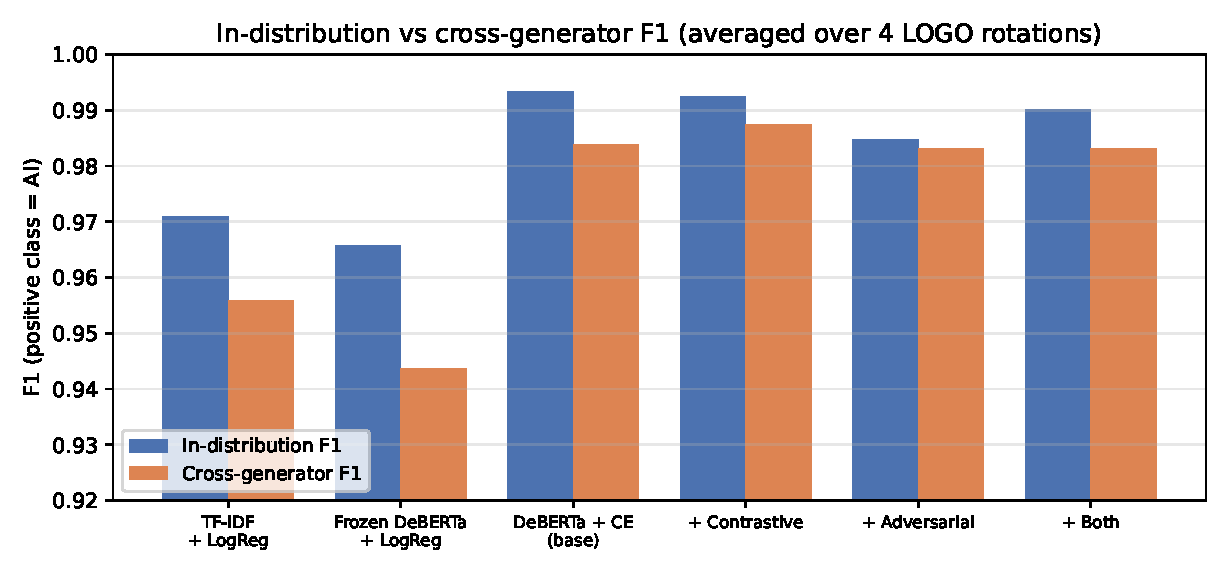
\includegraphics[width=0.92\textwidth]{f1_comparison.pdf}
\caption{In-distribution versus cross-generator F1 for the two baselines and the
four DeBERTa variants, averaged over the four LOGO rotations. Fine-tuned DeBERTa
closes most of the cross-generator gap that the baselines suffer.}
\label{fig:f1}
\end{figure}

\begin{figure}[t]
\centering
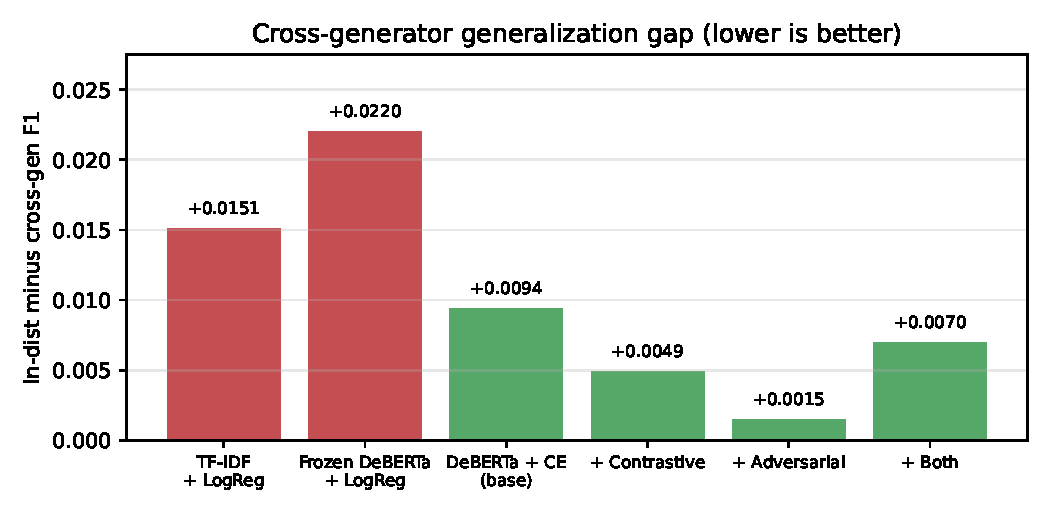
\includegraphics[width=0.78\textwidth]{gap.pdf}
\caption{Cross-generator generalization gap (in-distribution F1 minus
cross-generator F1) by model. The contrastive and adversarial objectives both
shrink the gap relative to plain cross-entropy.}
\label{fig:gap}
\end{figure}

\subsection{Per-held-out-generator breakdown}
Table~\ref{tab:pergen} and Figure~\ref{fig:pergen} break cross-generator F1 down
by which generator was held out. Gemma (rotation 2) is consistently the hardest
generator to catch unseen: plain cross-entropy drops to 0.9681 on held-out Gemma,
its worst rotation. Both representation-shaping objectives help most exactly
here, with contrastive raising held-out-Gemma F1 to 0.9808 and adversarial to
0.9815. GPT-5 mini and Qwen are the easiest to detect unseen, with all variants
above 0.98. This pattern explains why contrastive learning improves the average:
its largest gains land on the rotation where the base model is weakest.

\begin{table}[t]
\centering
\caption{Cross-generator F1 by held-out generator (one rotation each). Best
value in each row is in bold.}
\label{tab:pergen}
\begin{tabular}{clcccc}
\toprule
Rotation & Held out & CE & Contrastive & Adversarial & Both \\
\midrule
0 & gpt5mini & 0.9912 & \textbf{0.9902} & 0.9875 & 0.9844 \\
1 & deepseek & 0.9843 & \textbf{0.9861} & 0.9831 & 0.9802 \\
2 & gemma    & 0.9681 & 0.9808 & \textbf{0.9815} & 0.9754 \\
3 & qwen     & 0.9918 & \textbf{0.9930} & 0.9807 & 0.9926 \\
\bottomrule
\end{tabular}
\end{table}

\begin{figure}[t]
\centering
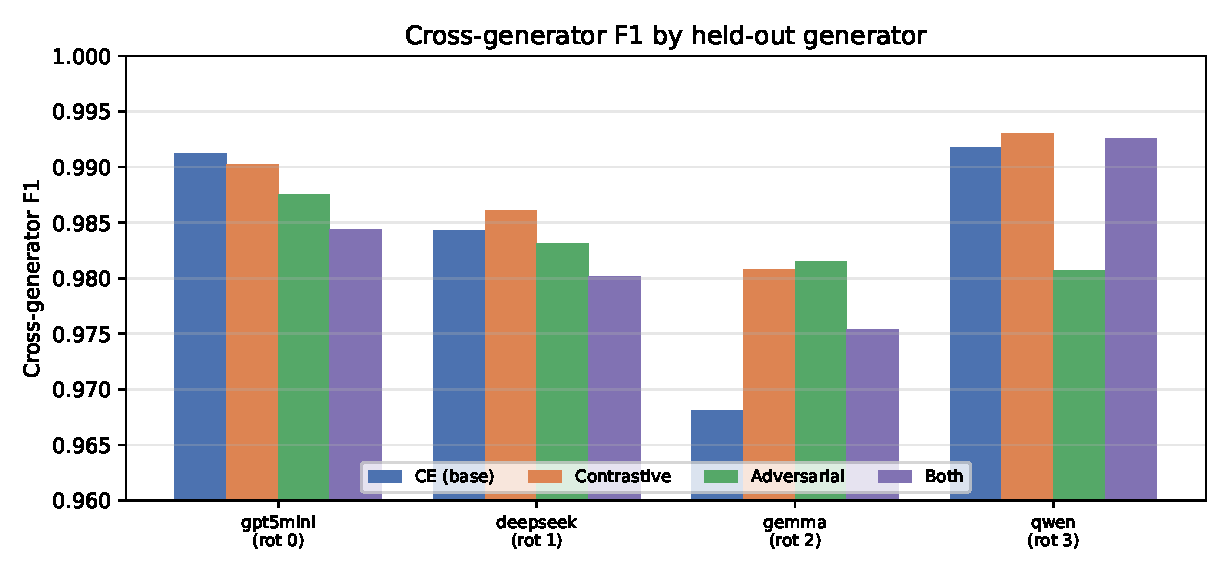
\includegraphics[width=0.92\textwidth]{per_generator.pdf}
\caption{Cross-generator F1 by held-out generator for the four DeBERTa variants.
Gemma (rotation 2) is the hardest to detect unseen, and it is where the
contrastive and adversarial objectives help most.}
\label{fig:pergen}
\end{figure}

\section{Discussion and Analysis}

\paragraph{Fine-tuning is what closes most of the gap.}
The single largest improvement in cross-generator F1 comes not from the
robustness objectives but from fine-tuning the encoder at all: cross-generator
F1 rises from 0.9437 (frozen probe) and 0.9558 (TF-IDF) to 0.9839 for plain
cross-entropy. A fine-tuned DeBERTa already learns a fairly
generator-invariant notion of AI writing in this corpus. The robustness
objectives then provide a second, smaller improvement on top.

\paragraph{Contrastive learning gives the best practical detector.}
The supervised contrastive variant is the one we would deploy. It has the highest
cross-generator F1 and AUC of any model, and it halves the generalization gap
relative to plain cross-entropy without the accuracy cost the adversarial variant
pays. Pulling all AI reviews into one cluster and all human reviews into another,
regardless of source, is exactly the inductive bias the cross-generator task
rewards, and its biggest gains appear on the hardest rotation (held-out Gemma).

\paragraph{Adversarial training minimizes the gap but not the error.}
The gradient-reversal variant produces the smallest gap (0.0015) precisely
because it lowers in-distribution F1 toward the cross-generator level rather than
raising cross-generator F1. Minimizing the gap is therefore not the same as
maximizing detection quality; a model that is uniformly mediocre has a small gap.
This is worth stating because the gap was our proposed headline metric: it should
be read together with absolute F1, not alone. Combining the two objectives did
not help, suggesting the adversarial gradient and the contrastive clustering work
against each other at these loss weights.

\paragraph{What the controlled setting does and does not show.}
Because target lengths were sampled from the human distribution and all
generators wrote about the same products, our gap reflects writing style, not
length or topic. That is the right design for the scientific question, but it
also makes detection easier than in the wild, where fake reviews often are
systematically shorter or longer and cluster on particular products. Our absolute
F1 numbers should be read as an upper bound on a controlled setting, not as
field performance.

\paragraph{Limitations.}
Several caveats apply. We substituted DeepSeek-V4-Flash for the proposal's IBM
Granite because Granite is not served through commodity hosted APIs, so our
results speak to the GPT-5 / DeepSeek / Gemma / Qwen family specifically. The
corpus is English-only. Three of four generators are reasoning models; although
we removed obvious reasoning traces, subtler stylistic artifacts of reasoning
models could remain and act as a shortcut feature. A single fixed prompt template
was used, whereas a real adversary would tune prompts, so our setting measures
detection of controlled, non-adversarial generation. Finally, each rotation's
cross-generator human pool is modest (about 2{,}470), which adds sampling noise
to the per-rotation cross-generator estimates, though it remains adequate for
F1 and AUC.

\section{Conclusion}

We studied whether an AI-review detector generalizes to generators it never saw
in training, using a controlled corpus of about 20{,}000 Amazon reviews and a
strict leave-one-generator-out protocol that holds product, topic, and length
fixed so the test isolates writing style. Fine-tuned DeBERTa-v3 generalizes far
better across generators than TF-IDF or frozen-feature baselines, and a
supervised contrastive objective is the best variant overall: it achieves the
highest cross-generator F1 (0.9875) and AUC (0.9994) and halves the
generalization gap relative to plain cross-entropy (0.0048 versus 0.0095). A
gradient-reversal adversarial objective minimizes the gap further (0.0015) but by
lowering in-distribution accuracy rather than raising cross-generator accuracy,
which shows that the gap must be read alongside absolute error. The hardest
generator to catch unseen is Gemma, and that is exactly where the
representation-shaping objectives help most. Future work should test against
genuinely held-out model families, prompt-tuned adversarial generation, and
non-English reviews, and should explore whether the contrastive and adversarial
objectives can be combined without the interference we observed.

\section*{Contribution Statement}

% TODO (Evan): fill in the contribution statement for each team member here.
\emph{Placeholder: describe each team member's contributions to data collection,
generation, split construction, model implementation, training, evaluation, and
the writing of this report.}

\begin{thebibliography}{9}

\bibitem{amazonreviews2023}
McAuley Lab.
\newblock Amazon Reviews 2023 dataset.
\newblock \url{https://huggingface.co/datasets/McAuley-Lab/Amazon-Reviews-2023}.

\bibitem{he2021deberta}
P.~He, X.~Liu, J.~Gao, and W.~Chen.
\newblock DeBERTaV3: Improving DeBERTa using ELECTRA-style pre-training with
gradient-disentangled embedding sharing.
\newblock \emph{arXiv:2111.09543}, 2021.

\bibitem{khosla2020supcon}
P.~Khosla, P.~Teterwak, C.~Wang, A.~Sarna, Y.~Tian, P.~Isola, A.~Maschinot,
C.~Liu, and D.~Krishnan.
\newblock Supervised contrastive learning.
\newblock In \emph{Advances in Neural Information Processing Systems (NeurIPS)},
2020.

\bibitem{ganin2015dann}
Y.~Ganin and V.~Lempitsky.
\newblock Unsupervised domain adaptation by backpropagation.
\newblock In \emph{International Conference on Machine Learning (ICML)}, 2015.

\bibitem{bag2025}
S.~Bag et al.
\newblock Detection of AI-generated reviews.
\newblock 2025.

\bibitem{guo2024}
B.~Guo et al.
\newblock How close is ChatGPT to human experts? Comparison corpus and
detection.
\newblock 2024.

\bibitem{kashifpour2025}
M.~Kashifpour et al.
\newblock LLM-generated text detection.
\newblock 2025.

\end{thebibliography}

\end{document}
